\chapter{Microarchitettura}

\section{Datapath}

Il ciclo di esecuzione di un processore è

\begin{lstlisting}[frame=single]
while(true) {
    Instruction = fetch(PC) // PC = program counter
    decode(Instruction)
    exec(Instruction)
    update(PC)
}
\end{lstlisting}

Vedremo come implementare un piccolo processore che esegue un sottoinsieme delle istruzioni ARM,
suddiviso in due oggetti, la parte di controllo e il \textbf{datapath} (parte operativa).

I processori possono essere di diversi tipi:
\begin{itemize}
    \item \textbf{Single cycle}: esegue un singolo ciclo fetch-decode-execute per ogni ciclo di clock (tutto viene eseguito nell'intervallo di tempo in cui il segnale di clock è basso).
    % //TODO schema
    \item \textbf{Multi cycle}: può eseguire un istruzione in più cicli di clock, in genere, un ciclo per il fetch-decode, un ciclo per l'exec e un ciclo per il writeback (risposta)
    % //TODO schema
    \item \textbf{Pipeline}:
\end{itemize}

\begin{note}
    \textbf{Prestazioni}

    La misura \textit{CPI} (Clock per Instruction) misura quanti cicli di clock $\tau$ sono necessari per eseguire un istruzione.
    Da tale misura possiamo dedurre, per ogni processore, il tempo necessario per eseguire un programma di $N$ istruzioni.
    Esso impiegherà $N \cdot CPI \cdot \tau $
\end{note}


\section{Processori Single Cycle}

Per realizzare un processore Single Cycle dobbiamo capire quali componenti (reti logiche e sequenziali) sono
necessari per realizzare il datapath. Possiamo inferire da i componenti necessari per mantenere lo stato del processore (Registri e memoria)
e l'insieme \textit{ISTR} di istruzioni che vogliamo implementare.

Vediamo i \textbf{componenti di stato}, il primo componente da utilizzare è una memoria per le istruzioni che riceverà in input
un indirizzo e restituirà in output l'\textbf{istruzione corrente}.

Il secondo componente necessario è una memoria dati (una RAM statica) che contiene la memoria sulla quale possiamo fare operazioni di \textit{load} e \textit{store}.
Ha bisogno di un solo indirizzo di memoria per la lettura e la scrittura, un input di clock, un input di \textit{write enable}, un indirizzo in input, un valore in input e un valore in output.

Il terzo componente necessario è una memoria multiporta statica che continene lo stato dei registri.
Riceverà in input 3 indirizzi (2 in lettura ed 1 in scrittura), un segnale di clock, uno di write enable, un valore in input e due in output.
Se il segnale \textit{write enable} è LOW, l'indirizzo in scrittura viene utilizzato per la lettura.
Sarà necessario un registro separato per mantenere il program counter, che riceverà sempre clock, write enable, input e restituirà il suo contenuto in output.

% //TODO schema dettagliato
% //TODO schema semplificato

\begin{defn}
\textbf{Implementare un'istruzione LDR (Load register)} \\
Vediamo come implementare un'istruzione \texttt{LDR} con offset immediato (pre-indice), prendiamo ad esempio
\begin{lstlisting}[style=arm]
ldr r0, [r1, #4]
\end{lstlisting}
Avremo il registro \texttt{pc} che punterà all'istruzione \texttt{ldr}. La memoria istruzioni conterrà l'istruzione all'indirizzo puntato da \texttt{pc}.
Caricheremo \texttt{r1} dal primo indirizzo di lettura della \textit{memoria registri} (nel suo output 1), a cui sommeremo  nella \textit{ALU} l'offset costante \texttt{\#4}.
Caricheremo dall'indirizzo sommato un valore dalla \textit{memoria dati}, che andrà in input alla memoria registri e verrà scritto all'indirizzo di scrittura,
in questo caso \texttt{r0}.
% //TODO SCHEMA
Se volessimo realizzare un offset variabile (un registro), come ad esempio
\begin{lstlisting}[style=arm]
ldr r0, [r1, r2]
\end{lstlisting}
Dovremmo utilizzare anche il secondo input/output di lettura della memoria registri, (il registro \texttt{r2}) come operando di somma della ALU.
Ciò ci fa notare che è necessario un multiplexer fra \textit{out2} della memoria registri e l'operando immediato per realizzare correttamente l'offset.
\end{defn}


\begin{defn}
\textbf{Implementare un'istruzione STR (Store register)} \\
Implementare un'istruzione di \textit{store} è simile all'implementazione di un istruzione di \textit{load}.
Il segnale \textit{write enable} della memoria registri sarà low. Leggerò dal primo output della memoria registri l'indirizzo in cui memorizzerò il valore,
dal secondo output della memoria registri il valore da memorizzare e opzionalmente, un registro di offset dal terzo output.
Il segnale \textit{write enable} della memoria dati sarà HIGH.
% //TODO ordine registri nella thumb
\end{defn}

\begin{defn}
\textbf{Implementare istruzioni di salto} \\
Per implementare le istruzioni di salto dobbiamo sommare un immediato
all'indirizzo corrente contenuto nel program counter, ed inserirlo di nuovo all'interno del program counter.
Abbiamo bisogno di un multiplexer posto fra l'uscita della memoria dati e l'uscita della ALU posta dopo gli output della memoria registri.
Collegheremo l'uscita di tale multiplexer all'ingresso del program counter, dove scriveremo il valore dell'istruzione dopo il salto.

Alla fine di un'istruzione \textit{non di salto} il program counter viene incrementato di 4 posizioni attraverso una ALU.
Ciò ci dice che è necessario avere un altro multiplexer in ingresso al program counter.
% //TODO
\end{defn}


\begin{figure}[htbp]
    \centering
    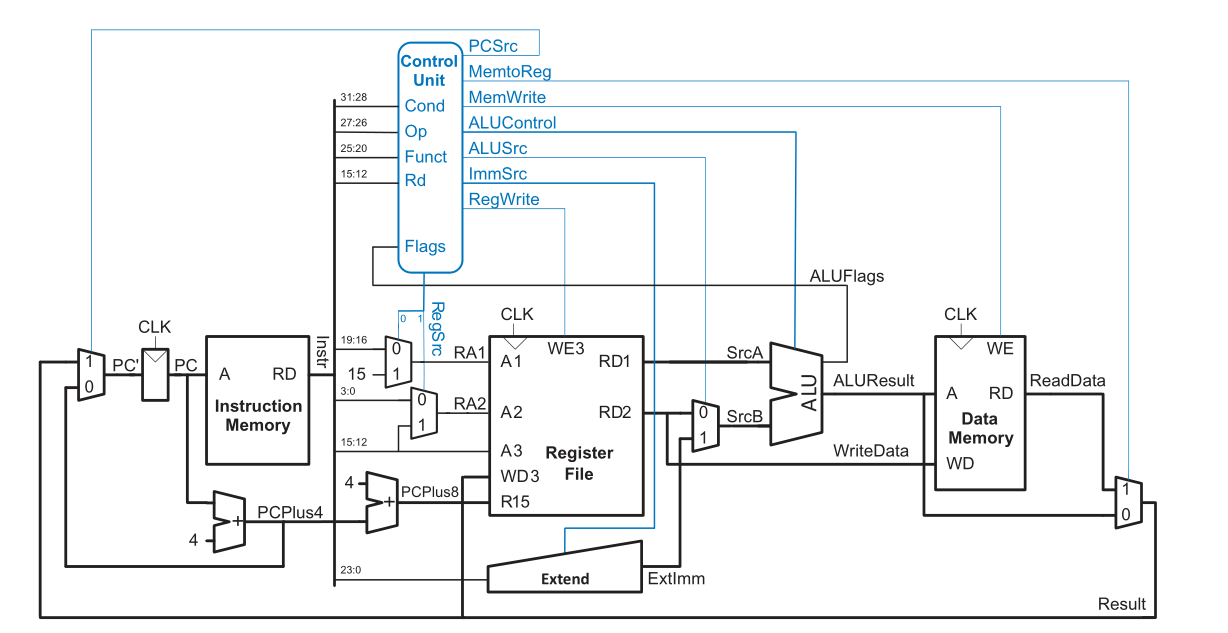
\includegraphics[width=1\textwidth]{completesinglecycleprocessor.png}
    \caption{Processore a ciclo singolo completo}
    \label{<label>}
\end{figure}